\documentclass[12pt]{article}
\usepackage{pck-english}
\usepackage{algorithmicx}
\usepackage{standalone}

\begin{document}

\subfile{forside.tex}

\section*{Abstract}
\label{sec:label}


\newpage
\section*{Acknowledgement}
\label{sec:ackow}

\newpage

\tableofcontents

\section{introduction}
\label{sec:intro}
\subsection{Background}
\label{subsec:label}
\subsection{Goal}
\label{subsec:label}






\section{Theory}
\label{sec:label}

\subsection{K-Means}
\label{subsec:kmeans}

K-means clustering is a method developed  of partitioning a set of points $X = \{x_1, x_2, ..., x_n\}$ in a d-dimensional space into a set of clusters $S = \{s_1, s_2, ..., s_k\}$, hence the name K-means. The algorithm takes n points and k number of clusters, it returns points split up into these clusters where an assignment has been made for each point to a given cluster. This problem is what is called a NP-hard problem this means that it's computationally hard. KMeans usually is one of the fastest clustering methods, but it suffers that it might converge to a local minimum instead of the sought after global minimum, but there are ways to more or less correct this fault.\cite{lloyd}

\subsection{Lloyd's Algorithm}
\label{subsec:lloyds}

The most common implementation of k-means is the so called Lloyd's Algorithm that uses an iterative refinement approach. To start of some initial centroids as the center of each cluster is called, is chosen at random, then at each iteration of the algorithm two steps are executed, and repeated until the individual clusters does not change anymore (This is called convergence), or is terminated by an upper bound of iterations. There are many methods for choosing the initial centroids, a common method is the Forgy method, where k random points of the input data set is chosen as the centroid. Another example is the KMeans++ method of initializing centroids, that aims to by careful seeding have a better start for the algorithm, and such reach convergence faster.\cite{plusplus} The two steps for each iteration can be outlined as such: \\

\textbf{Assignment:} For each data point, compute all distances to all centroids, and find the nearest one. assign this point to the cluster.\\
\textbf{Update:} For each cluster calculate the mean of all the assigned points to the cluster and move the cluster to the mean\\ \\

In a more strict notation it's as follow:

\begin{algorithm}[h!]
  \caption{Kmeans algorithm}
  \begin{algorithmic}

    \Procedure{Kmeans}{}
    \State $\textit{X} \gets \{x_1, x_2, .. x_n\}$
    \State $c_1, ..c_2,...,c_k \gets$ RANDOM(points, K)
    \While{not converged}
    \ForAll{ $x \in X$ }
    find $\phi_c(x)$ (closest centroids to x)
    \EndFor
    \ForAll{$c \in C$}
    $c =$ mean($\{x \in X | \phi_C(x) = c\}$)
    \EndFor
    \EndWhile

  \end{algorithmic}

\end{algorithm}

The algorithm has some problems, it has to compute the distance from each point to each cluster in each iteration, this takes computational power. To compute the distance between two points $p,q \in \mathbb{R}^d$ we have to do the following computation:

\begin{equation}
  L = ||p - q||^2 = (p_1 - q_1)^2 +...+(p_d - q_d)^2
\end{equation}
This is known as the euclidian distance, this can be written more compactly as

\begin{equation}
  L = \sqrt{\sum_{i=1}^d(p_i - q_i)^2}
\end{equation}
This gives d subtractions, d multiplications and d-1 sums, and then for comparison with the previous cluster calculate the following: $d_{min} > d$ \\
This evaluates to $3\cdot d$ calculations for each point and cluster. Thus for each iteration we would need to execute $3d \cdot n \cdot k$ operations.

\subsection{Convergence}
\label{subsec:Convergens}



\subsection{KMeans++}
When we initialize the clusters randomly, we don't know how well the clusters represent the optimal clusters that we are trying to find in the end, this may in some cases lead to some  bad centroids that takes a very long time to converge to til global minimum. Instead we want to use another method for initializing the centroids. For this purpose the kmeans++ algorithm was developed in 2007 by David Arthur and Sergei Vassilvitskii \cite{plusplus}.
First we let $D(x)$ denote the shortest (euclidean) distance from a data point $x$ to the closest centroids that we have already chosen. And we also define a probability as the following:
\begin{equation}
P(x) = \frac{D(x)^2}{\sum_{x\in X}D(x)^2}
\end{equation}
Then the algorithm is explained as such:
\begin{itemize}
  \item Take one center $c_1$ chosen at random from the set of points $X$
  \item Take a new center $c_i$ choosing $x\in X$ with probability $P(x)$.
  \item Repeat until we have k centers.
  \item Continue with normal KMeans
\end{itemize}

Here I have just pasted some of the original experimental results that David and Sergei found in their original paper.

\begin{table}[h!]
  \centering
    \begin{tabular}{|c| c |c| c| }
      & Average $\phi$ & Minimum $\phi$ & Average time (Seconds) \\
      k & Random KMeans++ & Random KMeans++ & Random KMeans++ \\
      \hline
      2&3&  ell8 & cell9
    \end{tabular}
    \caption{Table of results from original KMeans++ Paper.}
    \label{table:kpp}
\end{table}

The faster times the results show comes from the fact that with proper initialization of the centroids we reach convergence faster than with random initialized centroids. As discussed in \ref{subsec:lloyds} each iteration of the algorithm will need $3d \cdot n\cdot k$ operations, so decreasing the number of iterations will have a huge impact on performance.

\subsection{Bohrium}
\label{subsec:Bohrium}
Bohrium is framework that aims to present a way to speed-up array programming, it's a modular framework with support for multiple alternate front end and back ends. Bohrium was created in 2013, by Mads R. B. Kristensen

\subsection{How it works}
\label{subsec:hiw}
Bohrium lazily record any array operations that is used, this could as an example be from NumPy, and turn them into bytecode instruction set. An overview can be seen in figure \ref{fig:bohrium}

\begin{figure}[H]
  \centering
  \label{fig:bohrium}
  \documentclass{standalone}
\usepackage{tikz}
\begin{document}

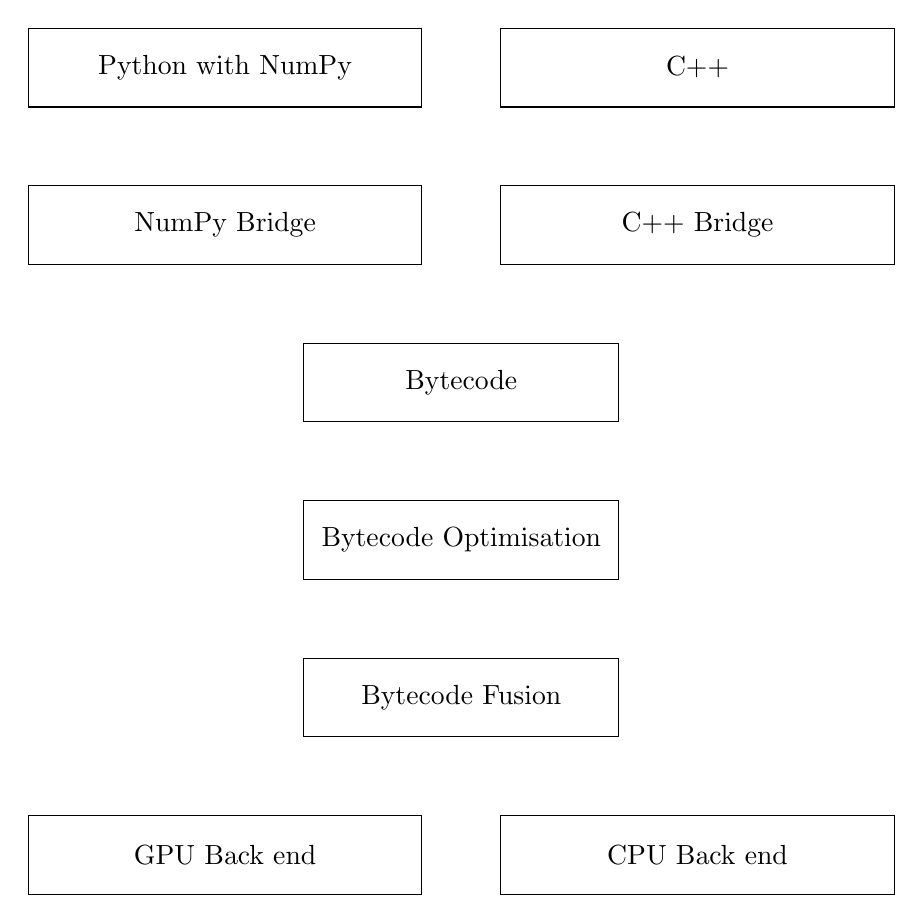
\begin{tikzpicture}
  \draw (1.5,0) rectangle (6.5, 1) node[pos=.5] {Python with NumPy};
  \draw (7.5,0) rectangle (12.5, 1) node[pos=.5] {C++};
  \draw (1.5,-1) rectangle (6.5, -2) node[pos=.5] {NumPy Bridge};
  \draw (7.5,-1) rectangle (12.5, -2) node[pos=.5] {C++ Bridge};

  \draw (5,-3) rectangle (9, -4) node[pos=.5] {Bytecode};
  \draw (5,-5) rectangle (9, -6) node[pos=.5] {Bytecode Optimisation};
  \draw (5,-7) rectangle (9, -8) node[pos=.5] {Bytecode Fusion};

  \draw (1.5,-9) rectangle (6.5, -10) node[pos=.5] {GPU Back end};
  \draw (7.5,-9) rectangle (12.5, -10) node[pos=.5] {CPU Back end};

\end{tikzpicture}

\end{document}

\caption{The components that Bohrium are made out of}
\end{figure}






\subsection{Vectorization}
\label{subsec:vectorization}

The point of vectorization is to generalize operations on scalars to apply on vectors, matrices and also higher-dimensional arrays. The idea is to do operations on an entire set of values instead of each single item in the set. As en example the operation of adding two arrays together in a scalar function would look like this implemented in python
\begin{lstlisting}[language=C]
  for (i=0; i < n; i++)
      for (j = 0; j < n; j++)
          a[index_a][index_b] += b[index_a][index_b]
\end{lstlisting}

This tedious way of coding can now be abstracted away, as more and more programming languages and libraries support what is known as array programming, as an example in the library for python called Numpy the code for adding to vectors together can the trivialized to $a + b = c$ this leads to simpler code and it makes it possible for the programmer to speak the same language as mathematicians.

Vectorized operations are typically allows for the operations to be run in parallel, thus speeding up the operation time. This in turn allows us further to run our code on GPU's which should lead to even greater speedups. These speedups will be discussed en greater detail when we discuss my vectorized implementation of the KMeans algorithm and my results.


\section{Implementation}
\label{subsec:implement}
\subsection{Overview}
\label{subsec:overview}
The program that was developed is aptly named Bohrium Kmeans, and as discussed is developed in Python using the Bohrium library for automatic GPU acceleration created by Mads. R. B. Kristensen. Bohrium Kmeans as most other kmeans implementations takes a set of points in any number of dimensions and number of clusters, this means that there is a large overlap in the way to use Bohrium Kmeans compared to some of the more popular libraries such as SKlearn for Python.\\
Bohrium Kmeans allows for alot of different parameters to be changed, as a concequence the user has control of how they want to use the program as an example they have the ability to choose how to initialize centroids, either by k-random centroids, first k-points or by the described kmeans++ algorithm.\\
In the following chapter I will desribe and detail some of the ways I implemented the algorithm and a chronological order and the issues and solutions i combated.
\subsection{Try: Only python}
\label{subsec:beginning}
To start of with the goal was to implement a barebones version of the kmeans algorithm in python without use of any external libraries, this decision means that we will have no array programming or vectorization. So we are left with only our knowledge of programming and a blank editor.
This means that we are forced to use loops in python, luckily python includes the feature: list comprehension which is a way of creating new list from  old list depending on some condition. This can get rid of some larger loops and as a bonus list comprehension is optimized for the python interpreter, just take a look this example where we choose k centroids from the set of points, first with a loop the standard way where we have to initialize the list to store the centroids in first, and then with a list comprehension.

\begin{lstlisting}[language=Python]
  centroids = []
  for i in range(k):
      centroids.append(points[randint(0, len(data)-1)])
\end{lstlisting}
Now with list comprehension
\begin{lstlisting}[language=Python]
centroids = [points[randint(0, len(data)-1)] for i in range(k)]
\end{lstlisting}
One way or the other we still loop sequentially k times and doing it this way is not vectorized thus we cannot hope to accelerate it in any meaningful way. A vectorized way will be discussed in the next chapter where start discussing the basic implementation using Numpy.
Another maybe even more surprising example, is the assignment step of Lloyd's algorithm where we have to compute the distance from each point to each centroid, without any vectorization we are again forced to use for loops, but this time a nested one

\begin{lstlisting}[language=Python]
  for p_idx, point in enumerate(points):
      distance_array = [0] * k #Initialize empty array
      for c_idx, centroids in enumerate(centroids):
          distance = euclidean_distance(point, centroid)
          distance_array[c_idx] = distance
      labels[p_idx] = distance_array.index(min(distance_array))
\end{lstlisting}

This is definitely hurtful for performance as we have to execute the body of the loop $n \times k$ times (not to mention the loop in the euclidean_distance function)




\subsection{Except: Numpy}
\label{subsec:middle}

\subsection{Finally: Bohrium}
\label{subsec:label}





\include{experiements}

\section{Conclusion}
\label{sec:label}


\bibliographystyle{plain}
\bibliography{ref,main}

\end{document}
